\section{Overview (Steering by Phase: A Quick Tour)}\label{sec:overview}

Picture ordinary motion as the wheels of a car and $\theta$ as a small, hidden steering column geared to them. Even on a perfectly flat road (no EM fields), turning the hidden column and coming back to where you started leaves a loop holonomy that interferometers can read. If the gear ratio varies across space (mixed curvature $G_{\mu\theta}$), the car drifts sideways (a cross-Hall response). The dial is periodic: turn it by $2\pi$ and the effects repeat.

Three lab anchors: (i) $\theta$--Aharonov--Bohm at $\mathbf E=\mathbf B=0$, (ii) cross-Hall drift from $\partial_i A_\theta$, and (iii) rotor sidebands with spacing $\Delta E\approx\hbar^2/(2I)$.

\begin{figure}[h]
  \centering
  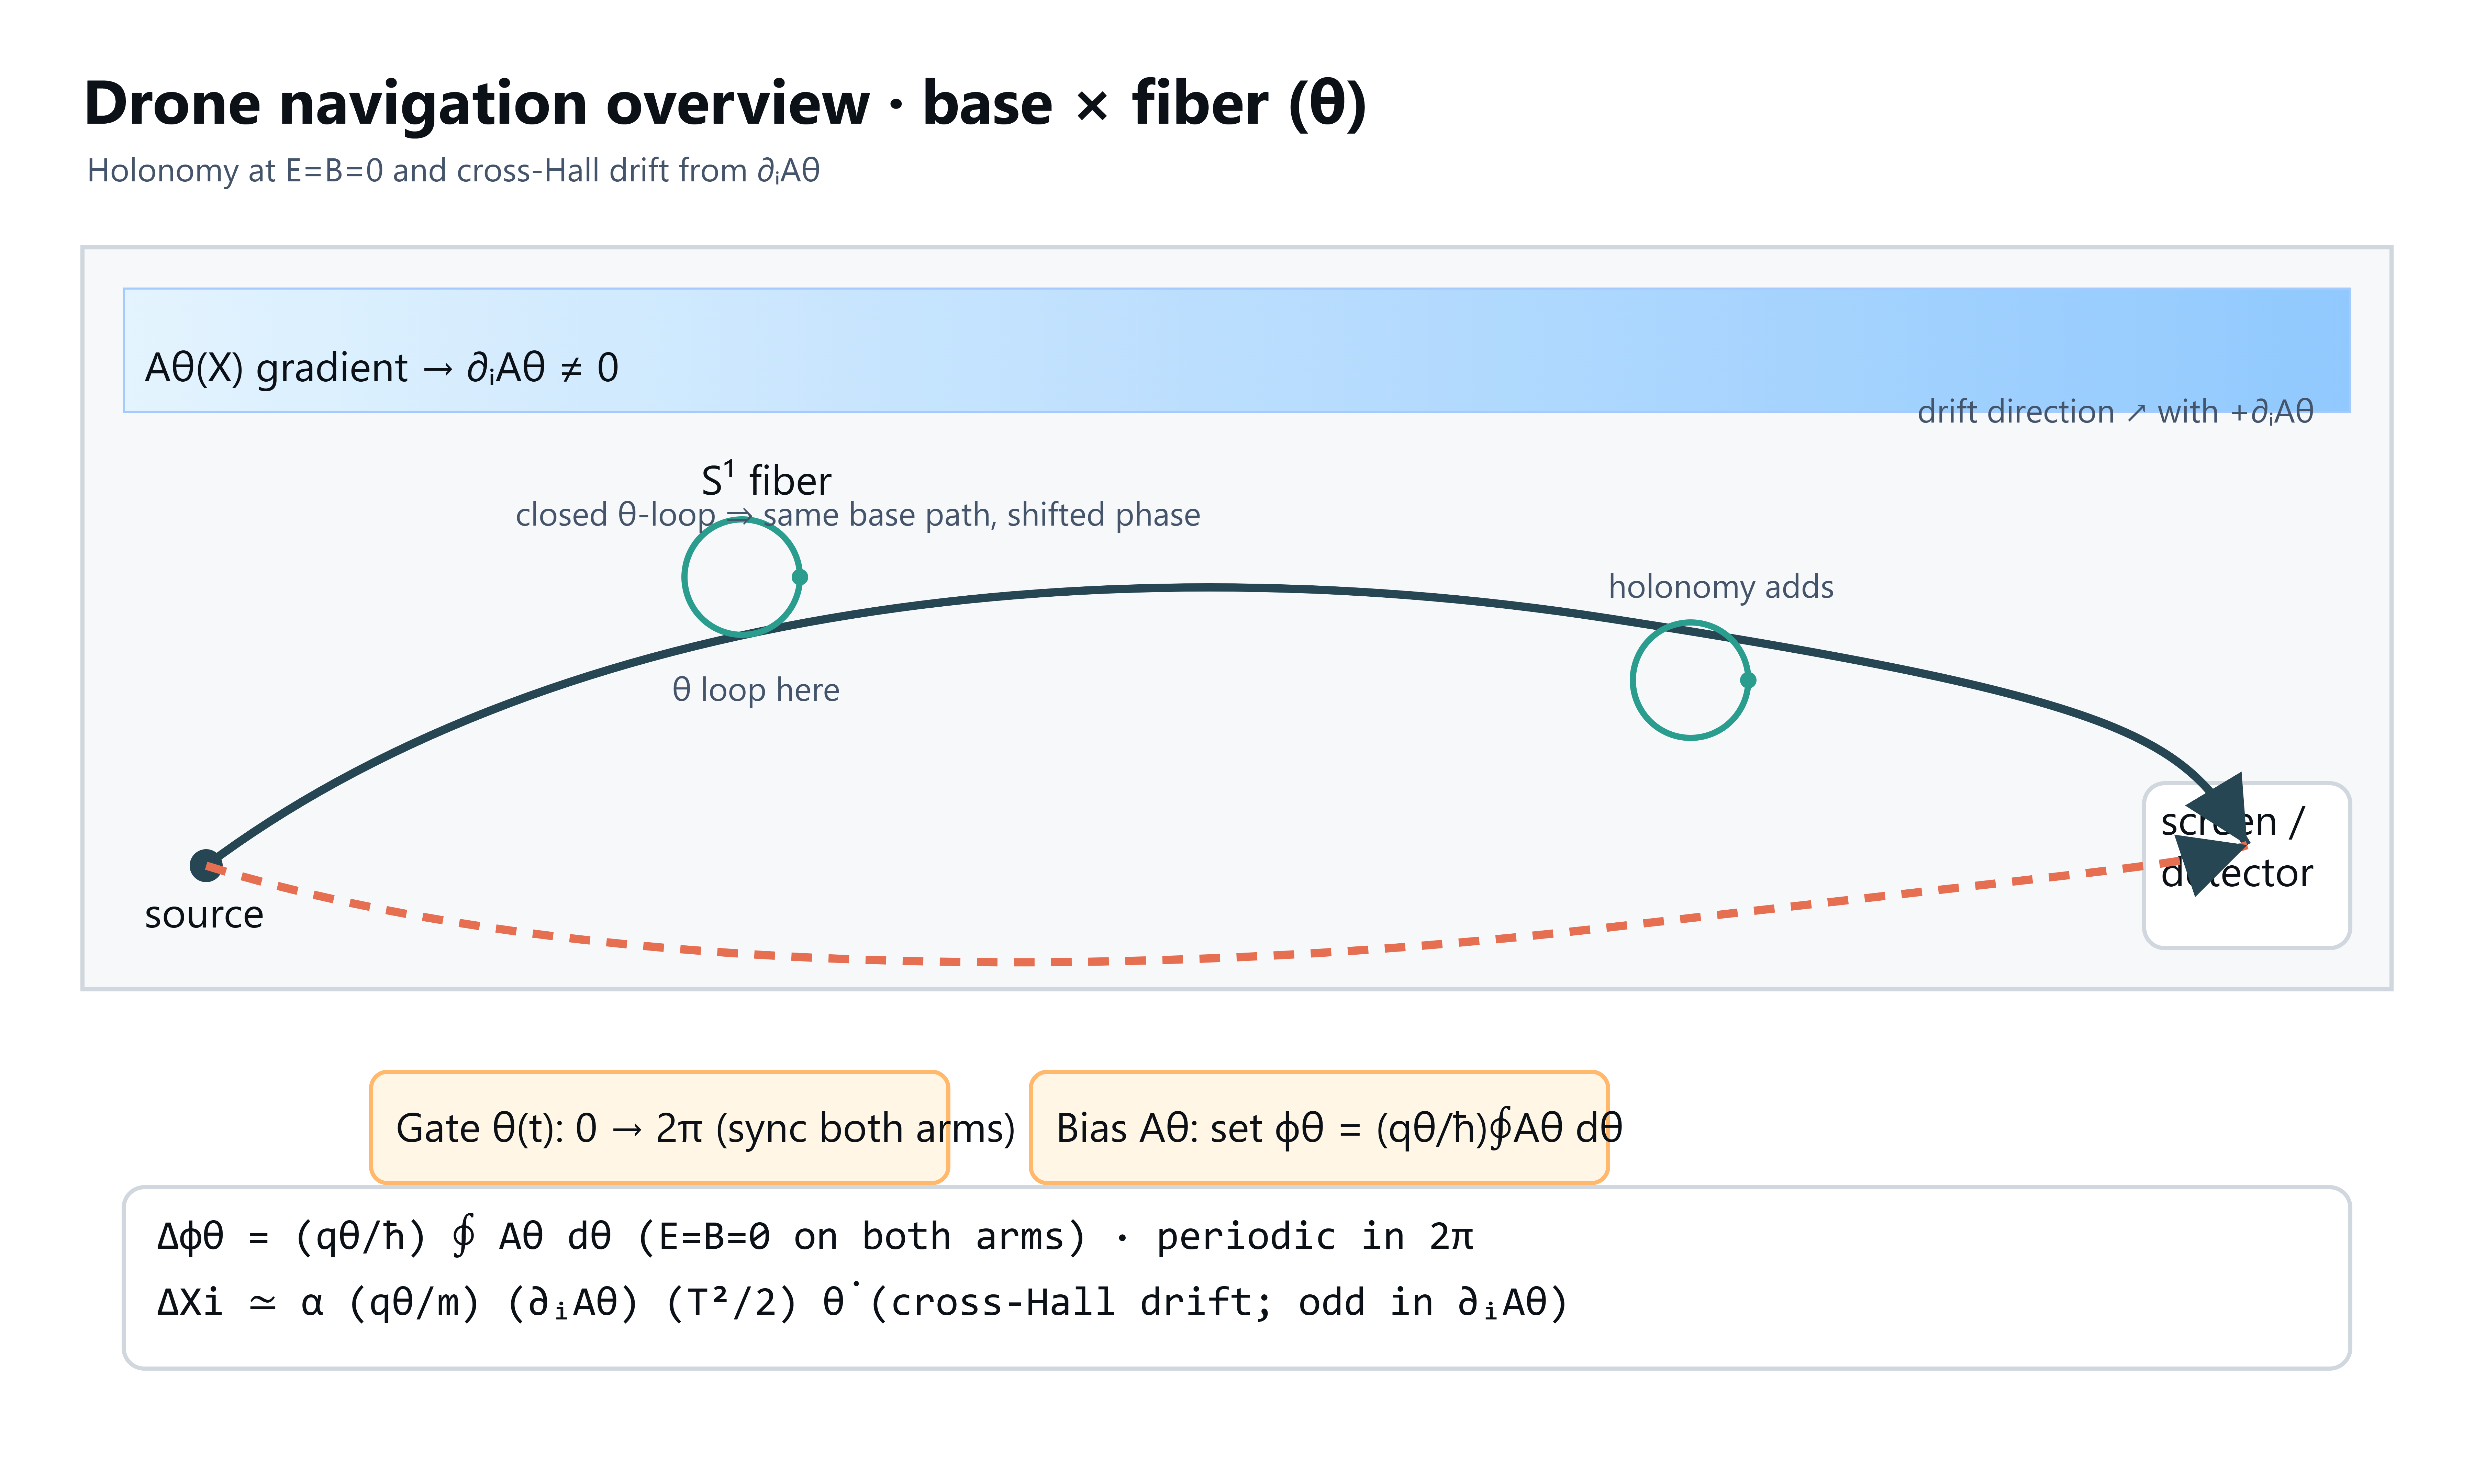
\includegraphics[width=0.75\linewidth]{drone_nav_overview.png}
  \caption{Drone navigation analogy: base motion (drone) with an internal $\theta$ dial (orange). Closing a loop on the dial leaves a holonomy $\phi_\theta$ visible at $\mathbf E=\mathbf B=0$; blue arrows illustrate cross-Hall drifts when $\partial_\mu A_\theta\neq 0$.}
  \label{fig:drone-analogy}
\end{figure}

Pointers: lab holonomy (\cref{sec:theta-ab}), sidebands as an inertia gauge (\cref{sec:sidebands}), unified range (\cref{sec:unified-force}), and bounce/WDW barrier (\cref{sec:cosmology}).
